\documentclass[11pt]{article}%{scrartcl}
\usepackage[scale=1.5]{ccicons}
\usepackage[notextcomp]{kpfonts} 
\usepackage[margin=1in]{geometry}
\usepackage{amsthm,amssymb}
\usepackage{graphicx}
\usepackage{enumitem}
\usepackage{bm}
\usepackage{ulem}
\usepackage{tikz}

\usepackage{color}
\definecolor{darkblue}{rgb}{0, 0, .6}
\definecolor{grey}{rgb}{.7, .7, .7}
\usepackage[breaklinks]{hyperref}
\hypersetup{
	colorlinks=true,
	linkcolor=darkblue,
	anchorcolor=darkblue,
	citecolor=darkblue,
	pagecolor=darkblue,
	urlcolor=darkblue,
	pdftitle={},
	pdfauthor={}
}

\usepackage{fancyhdr}
\pagestyle{fancy}
\lhead{MAT 526 - Spring 2021}
\chead{}
\rhead{Due \sout{Monday, January 25} Tuesday, January 26}
%\lfoot{}%\scriptsize This work is licensed under the \href{http://creativecommons.org/licenses/by-sa/3.0/us/}{Creative Commons Attribution-Share Alike 3.0 License}.} 
%\cfoot{}
%\rfoot{\ccbysa}
\renewcommand{\headrulewidth}{.4pt}
%\renewcommand{\footrulewidth}{.4pt}

\theoremstyle{definition}
\newtheorem{theorem}{Theorem}
\newtheorem{acknowledgement}[theorem]{Acknowledgement}
\newtheorem{algorithm}[theorem]{Algorithm}
\newtheorem{axiom}[theorem]{Axiom}
\newtheorem{case}[theorem]{Case}
\newtheorem{claim}[theorem]{Claim}
\newtheorem*{claim*}{Claim}
\newtheorem{conclusion}[theorem]{Conclusion}
\newtheorem{condition}[theorem]{Condition}
\newtheorem{conjecture}[theorem]{Conjecture}
\newtheorem{corollary}[theorem]{Corollary}
\newtheorem{criterion}[theorem]{Criterion}
\newtheorem{definition}[theorem]{Definition}
\newtheorem{example}[theorem]{Example}
\newtheorem{exercise}[theorem]{Exercise}
\newtheorem{journal}[theorem]{Journal}
\newtheorem{lemma}[theorem]{Lemma}
\newtheorem{notation}[theorem]{Notation}
\newtheorem{problem}[theorem]{Problem}
\newtheorem{proposition}[theorem]{Proposition}
\newtheorem{remark}[theorem]{Remark}
\newtheorem{solution}[theorem]{Solution}
\newtheorem{summary}[theorem]{Summary}
\newtheorem{skeleton}[theorem]{Skeleton Proof}
\newtheorem{activity}[theorem]{Activity}
\newtheorem{intuitivedef}[theorem]{Intuitive Definition}

\newcommand{\blankline}{\pagebreak[2]\vspace{.5\baselineskip}}

\setlength{\parindent}{0pt}

%Useful for cut and paste
%\begin{enumerate}[label=\rm{(\alph*)}]

\begin{document}

\begin{center}
{\Large\bf Homework 4}

\smallskip

Combinatorics
\end{center}

\thispagestyle{fancy}

You are allowed and encouraged to work together on homework. Yet, each student is expected to turn in their own work. In general, late homework will not be accepted. However, you are allowed to turn in \textbf{up to two late homework assignments with no questions asked}. When doing your homework, I encourage you to consult the \href{http://danaernst.com/teaching/ElementsOfStyle.pdf}{Elements of Style for Proofs}. Unless otherwise indicated, submit each of the following assignments via BbLearn by the due date. You will need to capture your handwritten work digitally and then upload a PDF to BbLearn. There are many free smartphone apps for doing this. I use TurboScan on my iPhone.

\blankline

Reviewing material from previous courses and looking up definitions and theorems you may have forgotten is fair game. However, when it comes to completing assignments for this course, you should \textit{not} look to resources outside the context of this course for help.  That is, you should not be consulting the web, other texts, other faculty, or students outside of our course in an attempt to find solutions to the problems you are assigned.  This includes Chegg and Course Hero. On the other hand, you may use each other, the textbook, me, and your own intuition. \textbf{If you feel you need additional resources, please come talk to me and we will come up with an appropriate plan of action.} Please read NAU's \href{https://www5.nau.edu/policies/Client/Details/828?whoIsLooking=Students&pertainsTo=All&sortDirection=Ascending&page=1}{Academic Integrity Policy}.

\blankline

Complete the following problems. 
\begin{enumerate}
%\item Let $s_n$ denote the number of subsets of $[n]$ that contain no two consecutive elements.  Determine $s_n$ in terms of a recurrence or a closed form, or by describing a bijection to a set we already know how to count.
\item An L-tiling of a $2\times n$ rectangle is like a domino tiling except it uses the following pieces, which are allowed to be rotated:
\begin{center}
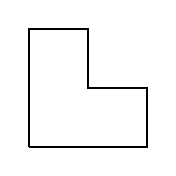
\begin{tikzpicture}[scale=.75]
\draw[thick] (0,0) to (2,0) to (2,1) to (1,1) to (1,2) to (0,2) to (0,0);
\end{tikzpicture}
\hspace{1cm}

\begin{tikzpicture}[scale=.75]
\draw[thick] (0,0) rectangle (1,1);
\end{tikzpicture}
\end{center}
Let $\ell_n$ denote the number of L-tilings of a $2\times n$ rectangle.  We can take $\ell_0=1$.  Compute $\ell_1$ and $\ell_2$ and then find a recurrence for $\ell_n$ for $n\geq 3$.
\item \textbf{Updated!} Let $F_n$ denote the number of tilings of a $1\times n$ array as described in Problem 8 on Homework 3.  Prove that for $m\geq 3$ and $n\geq 2$, we have $F_{m+n-1}=F_{m-2}F_{n-1}+F_{m-1}F_{n}$. \textit{Hint:} By definition, the lefthand side counts the number of tilings of an array with $m+n-1$ entries.  So, it suffices to show that the righthand side counts the same thing.  Number the entries 1 through $m+n-1$, from left to right. Let $\mathcal{S}_m$ be the collection of tilings where there is a $1\times 2$ tile covering the entries labeled by $m-1$ and $m$, and let $\mathcal{T}_m$ be the collection of tilings where this is not the case.  Does this tell us anything about the Fibonacci sequence?
\item Complete Problem 1.4.
\item What are the alternating row sums in Pascal's Triangle?  That is, for $n\geq 0$, find a formula for $\sum_{k=0}^{n}(-1)^k\binom{n}{k}$. Instead of using the Binomial Theorem, find a proof that either uses the meaning of $\binom{n}{k}$ or rearrange the sum and use the symmetry theorem (i.e., $\binom{n}{k}=\binom{n}{n-k}$). You might want to consider the cases for $n$ odd versus even separately.
%\item What are the diagonal sums in Pascal's Triangle.  That is, find a formula for $\sum_{k\geq 0}\binom{n-k}{k}$. Note that the sum ends after about $n/2$ terms since $\binom{a}{b}=0$ if $b>a$. 
\item Prove that for any $k$ and $m$ less than or equal to $n$, we have $\binom{n}{k}=\sum_{j=0}^k\binom{n-m}{j}\binom{m}{k-j}$. \textit{Hint:} Split $[n]$ into two piles, say $A_m=\{1,\ldots,m\}$ and $B_m=\{m+1,\ldots,n\}$. For each $j\in\{0,\ldots, k\}$, count number of ways to get a $k$-subset by selecting the appropriate number from $A_m$ and the appropriate number from $B_m$.
\item In calculus, the Power Rule for Derivatives states that
\[
\frac{d}{dx}\left[x^n\right]=nx^{n-1}.
\]
Moreover, the definition of the derivative tells us that
\[
\frac{d}{dx}\left[x^n\right]=\lim_{h\to 0}\frac{(x+h)^n-x^n}{h}.
\]
Using the Binomial Theorem, prove the Power Rule in the case when $n$ is a positive integer.
\item Use the Binomial Theorem to find a formula for $\sum_{k=0}^n2^k\binom{n}{k}$.
\item Use the Binomial Theorem to find a formula for $\sum_{k=0}^n(-2)^k\binom{n}{k}$.
\end{enumerate}
\end{document}